\chapter*{Exercises C6}

\begin{enumerate}

	\item \begin{subequations}
		\begin{enumerate}
			\item Let $ Y = (X_1 + X_2) / 2 $. This gives the following joint PMF for $ Y $,\\
			\begin{table}[H]
				\centering
				\begin{tabular}{@{}rrrrr@{}}
					\toprule
					 &     $ X_1 =  $0 &     $ X_1 =  $1 &    $ X_1 =  $2 &     $ X_1 =  $3 \\
					\midrule
					$ X_2 =  $0 &  0.04 &  0.06 &  0.0 &  0.10 \\
					$ X_2 =  $1 &  0.06 &  0.09 &  0.0 &  0.15 \\
					$ X_2 =  $2 &  0.00 &  0.00 &  0.0 &  0.00 \\
					$ X_2 =  $3 &  0.10 &  0.15 &  0.0 &  0.25 \\
					\bottomrule
				\end{tabular}
			\end{table}

			\begin{table}[H]
				\centering
				\begin{tabular}{@{}rrrrr@{}}
					\toprule
					$ i $ &     $P\left\{Y = i\right\}$ \\
					\midrule
					0 &  0.04  \\
					1/2 &  0.12  \\
					1 &  0.09  \\
					3/2 &  0.20  \\
					2 & 0.30 \\
					5/2 & 0.00 \\
					3 & 0.25 \\
					\bottomrule
				\end{tabular}
			\end{table}
		
		\item \begin{align}
			\mathbb{E}[Y] &= \sum\limits_{i} i\ \times P\left\{Y = i\right\} = 1.8 \\
			%
			\mathbb{E}[Y^2] &= \sum\limits_{i} i^2\ \times P\left\{Y = i\right\} = 4.02 \nonumber \\
			%
			\mathrm{Var}(Y) &= 4.02 - (1.8)^2 = 0.78
		\end{align}\\
	
		Alternatively, using the new sample mean and variance formulae, \\
		
		\begin{align}
			\mathbb{E}[X_i] &= 1.8 & \mathrm{Var}(X_i) &= 4.8 - 1.8^2 = 1.56 \\
			%
			\mathbb{E}[\overline{X}] &= \mathbb{E}[X_i] = 1.8  &\mathrm{Var}(\overline{X}) &= \mathrm{Var}(X_i) / 2 = 0.78
		\end{align}\\
	
		\item Let $ Z = (X_1 + X_2 + X_3) / 3 $. The PMF of $ Z $ is given by \\
		\begin{table}[H]
			\centering
			\begin{tabular}{@{}rrrrr@{}}
				\toprule
				$ i $ &     $P\left\{Z = i\right\}$ \\
				\midrule
				0 &  0.008  \\
				1/3 &  0.036  \\
				2/3 &  0.054  \\
				1 &  0.087  \\
				4/3 & 0.18 \\
				5/3 & 0.135 \\
				2 & 0.15 \\
				7/3 & 0.225 \\
				8/3 & 0 \\
				3 & 0.125 \\
				\bottomrule
			\end{tabular}
		\end{table}
	
		\item Using the new sample mean and variance formulae, \\
		
		\begin{align}
			\mathbb{E}[X_i] &= 1.8 & \mathrm{Var}(X_i) &= 4.8 - 1.8^2 = 1.56 \\
			%
			\mathbb{E}[\overline{Z}] &= \mathbb{E}[X_i] = 1.8  &\mathrm{Var}(\overline{Z}) &= \mathrm{Var}(X_i) / 3 = 0.52
		\end{align}\\
		\end{enumerate}
	\end{subequations}

	\item 10 fair dice are rolled. Let the dice be $ \left\{X_i\right\} $. Now, $ Y = \sum_{i} X_i  $
	
	\begin{subequations}
		\begin{align}
			\mathbb{E}[X_i] &= 3.5 		& \mathrm{Var}(X_i) &= 91/6 - 49/4 = 35/12 \nonumber \\
			%
			\mathbb{E}[Y] &= 35 		& \mathrm{Var}(Y) &= 350/12 
		\end{align}
	
		Using central limit theorem with continuity correction, \\
		\begin{align}
			P\left\{29.5 \leq Y \leq 40.5 \right\} &= P\left\{\frac{29.5 - 35}{\sqrt{350/12}} \leq Z \leq \frac{40.5 - 35}{\sqrt{350/12}}\right\} \nonumber \\
			%
			&= \Phi \left( \frac{40.5 - 35}{\sqrt{350/12}} \right) - \Phi\left(\frac{29.5 - 35}{\sqrt{350/12}}\right) = 0.6915
		\end{align} \\
	\end{subequations}

	\item 16 independent standard uniform RV. Let $ Y = \sum X_i  $. \\
		\begin{subequations}
			\begin{align}
				P \left\{Y > 10 \right\} &= P \left\{ \overline{X} > 10/16 \right\} \nonumber \\
				%
				&= P \left\{ \frac{4\ (\overline{X} - 0.5)}{\sqrt{1/12}}> \frac{1/2}{\sqrt{1/12}} \right\} \nonumber \\
				%
				&= 1 - \Phi\left( \frac{1/2}{\sqrt{1/12}} \right) = 0.0416
			\end{align}\\
		\end{subequations}
	
	\item \begin{subequations}
		\begin{enumerate}
			\item Each bet is independent with probability of success $ p = 1/38 $. Let $ Y = \sum X_i $\\
			\begin{align}
				\mathbb{E}[X] &= 35 \times 1/38 + (-1) \times 37/38 = -1/19 \\
				%
				\mathbb{E}[X^2] &= 35^2 \times 1/38 + (-1)^2 \times 37/38 = 631/19 \nonumber \\
				%
				\mathrm{Var}(X) &= 630/19 = 33.16 \\
				%
				\mathbb{E}[Y] &= n\mu \qquad \mathrm{Var}(Y) = n\sigma^2 \nonumber \\
				%
				P \left\{ Y > 0 \right\} &= 1 - \Phi \left( \frac{0 - n\mu}{\sqrt{n\sigma^2}} \right) \nonumber
			\end{align}\\
			
			\item The fact that the expected value of a single bet is negative means that it is more difficult to remain positive as the number of bets increases.
			\begin{align}
				n = 34 &\to P \left\{ Y > 0 \right\} = 0.4787 \nonumber \\
				%
				n = 1000 &\to P \left\{ Y > 0 \right\} = 0.3863 \nonumber \\
				%
				n = 100000 &\to P \left\{ Y > 0 \right\} = 0.0019 \nonumber
			\end{align}\\
		\end{enumerate}
	\end{subequations} 

	\item $ X_i $ is an RV with $ \mu = 1.5 $ and $ \sigma = 0.3 $. Assume \\
		\begin{subequations}
			\begin{enumerate}
				\item $ n = 50 $
				\begin{align}
					\mathbb{E}[Y] &= n\mu \qquad \mathrm{Var}(Y) = n\sigma^2 \nonumber \\
					%
					P \left\{ Y \leq 80 \right\} &= P \left\{Z \leq \frac{80 - n\mu}{\sqrt{n\sigma^2}} \right\} \nonumber \\
					%
					&= \Phi \left(\frac{80 - 75}{\sqrt{50\ (0.3)^2}}\right) = 0.9908
				\end{align}\\
				
				\item Assume snowfall on each day is independent.\\
				
				\item Assumption is bad since current weather events are usually dependent on the weather conditions of the past days.\\

			\end{enumerate}
		\end{subequations} 
	
	\item 50 independent uniform RV in the range $ [-0.5, 0.5] $. Let $ Y = \sum X_i  $. \\
		\begin{subequations}
			\begin{align}
				P \left\{Y > 3 \right\} &= P \left\{ \overline{X} > 0.06 \right\} \nonumber \\
				%
				&= P \left\{ \frac{\sqrt{50}\ (\overline{X} - 0)}{\sqrt{1/12}}> \frac{0.06 \sqrt{50}}{\sqrt{1/12}} \right\} \nonumber \\
				%
				&= 1 - \Phi\left( \frac{0.06 \sqrt{50}}{\sqrt{1/12}} \right) = 0.0708 \nonumber \\
				%
				P \left\{|Y| > 3 \right\} &= 2 \times P \left\{Y > 3 \right\} = 0.1416
			\end{align}\\
		\end{subequations}
	
	\item $ \mu = 7/2 $ and $ \sigma^2 = 35/12 $. Let $ n = 140 $ , Let $ Y = \sum X_i $\\
	\begin{subequations}
		\begin{align}
			P \left\{Y < 400 \right\} &= P \left\{ Z < \frac{(400 - 490)}{\sqrt{35/12 \times 140}} \right\} \nonumber \\
			%
			&= \Phi (-4.4538) \approx 0
		\end{align}\\
	\end{subequations}

	\item $ \mathbb{E}[X_i] = 5 $ and $ \mathrm{Var}(X_i) = 2.25 $. Lifetime of 12 batteries has to be less than a year.\\
	Let $ Y = \sum^n_1 X_i $. At $ n = 12 $ , \\
	\begin{subequations}
		\begin{align}
			P \left\{Y < 52 \right\} &= P \left\{ \overline{X} \leq 52/12 \right\} \nonumber \\
			%
			&= P \left\{ Z \leq \frac{\sqrt{12}\ (52/12 - 5)}{1.5} \right\} \nonumber \\
			%
			&= 0.0618 \nonumber 
		\end{align}\\
	\end{subequations}
	
	\item $ \mu = 100 $ and $ \sigma = 20 $. Let $ n = 16 $ , \\
	\begin{subequations}
		\begin{align}
			P \left\{\overline{X} < 104 \right\} &= P \left\{ Z < \frac{\sqrt{16}\ (104 - 100)}{20} \right\} \nonumber \\
			%
			&= \Phi (0.8) = 0.7881 \\
			%
			P \left\{98 < \overline{X} < 104 \right\} &= P \left\{ \frac{\sqrt{16}\ (98 - 100)}{20} < Z < \frac{\sqrt{16}\ (104 - 100)}{20} \right\} \nonumber \\
			%
			&= \Phi (0.8) - \Phi(-0.4) = 0.4436
		\end{align}\\
	\end{subequations}

	\item $ \mu = 2.2 $ and $ \sigma = 0.3 $. Let $ n = 100 $ , \\
	\begin{subequations}
		\begin{align}
			P \left\{\overline{X} > 3.1 \right\} &= P \left\{ Z > \frac{\sqrt{100}\ (3.1 - 2.2)}{0.3} \right\} \nonumber \\
			%
			&= 1 - \Phi (9/0.3) \approx 0  
		\end{align}\\
	\end{subequations}

	\item $ \mu = 500 $ and $ \sigma = 80 $. Let $ n $ vary and check probability, \\
	\begin{subequations}
		\begin{align}
			P \left\{\overline{X} > 525 \right\} &= P \left\{ Z > \frac{\sqrt{n}\ (525 - 500)}{80} \right\} \\
			%
			n = 4 &\to P = 1 - \Phi(5/8) = 0.266 \nonumber \\
			%
			n = 16 &\to P = 1 - \Phi(5/4) = 0.1056 \nonumber \\
			%
			n = 36 &\to P = 1 - \Phi(15/8) = 0.0304 \nonumber \\
			%
			n = 64 &\to P = 1 - \Phi(2.5) = 0.00621 \nonumber 
		\end{align}\\
	\end{subequations}
	
	\item $ \mu = 77$ and $ \sigma = 15 $. Let $ n = 25, 64 $ for the class average test scores $ Y, Z $ respectively, \\
	\begin{subequations}
		\begin{enumerate}
			\item \begin{align}
				P \left\{72 < Y < 82 \right\} &= P \left\{ \frac{\sqrt{25}\ (72 - 77)}{15} Z < \frac{\sqrt{25}\ (82 - 77)}{15} \right\} \nonumber \\
				%
				&= \Phi (5/3) - \Phi (-5/3) = 0.9044
			\end{align}\\
		
			\item \begin{align}
				P \left\{72 < Z < 82 \right\} &= P \left\{ \frac{\sqrt{64}\ (72 - 77)}{15} Z < \frac{\sqrt{64}\ (82 - 77)}{15} \right\} \nonumber \\
				%
				&= \Phi (8/3) - \Phi (-8/3) = 0.9923
			\end{align}\\
		
			\item Let $ W = Y - Z $, now, $ \mathbb{E}[W] = 0$, and $ \mathrm{Var}(W) = \sigma^2 (1/25 + 1/64) $\\
			\begin{align}
				P \left\{Y > Z \right\} &= P \left\{ W > 0 \right\} = \left\{ Z > \frac{(0 - 0)}{\sqrt{15*89/1600}} \right\} \nonumber \\
				%
				&= \Phi (0) = 0.5
			\end{align}\\
		
			\item The larger class has a smaller variance and is therefore, less likely have an average far from the mean. Thus, the smaller class is likelier to have a class average of 83.
		\end{enumerate}
	\end{subequations}

	\item Binomial RV with $ n = 150$ and $ p = 0.6 $. \\
	\begin{subequations}
		\begin{enumerate}
			\item \begin{align}
				P \left\{X \leq 80 \right\} &=  \sum\limits_{k=0}^{80} \binom{150}{k}\ 0.6^k\ 0.4^{1-k}\nonumber \\
				%
				&= 0.05746
			\end{align}\\
			
			\item approximating using normal RV without continuity correction, \\
			\begin{align}
				P \left\{X \leq 80 \right\} &= P \left\{ \frac{X - np}{\sqrt{np(1-p)}} \leq \frac{(80 - 90)}{6} \right\} \nonumber \\
				%
				&= 0.04779
			\end{align}\\
			
			\item with continuity correction\\
			\begin{align}
				P \left\{X \leq 80.5 \right\} &= P \left\{ \frac{X - np}{\sqrt{np(1-p)}} \leq \frac{(80.5 - 90)}{6} \right\} \nonumber \\
				%
				&= 0.056673
			\end{align}\\
		\end{enumerate}
	\end{subequations}
	
	\item Let $ A_2, A_3, A_4 $ denote the number of games that $ A $ wins against $ B, C, D $ respectively.\\
	\begin{subequations}
		\begin{enumerate}
			\item Looking at a table of the win probabilities,\\
			
			\begin{table}[H]
				\centering
				\begin{tabular}{@{}l|rrrr@{}}
					\toprule
					{} &     A &    B &    C &     D \\
					\midrule
					A &  0.00 &  0.6 &  0.7 &  0.75 \\
					B &  0.40 &  0.0 &  0.6 &  0.70 \\
					C &  0.30 &  0.4 &  0.0 &  0.50 \\
					D &  0.25 &  0.3 &  0.5 &  0.00 \\
					\bottomrule
				\end{tabular}
			\end{table}
		
			\begin{align}
				\mathbb{E}[A] &= \mathbb{E}[A_1] + \mathbb{E}[A_2] + \mathbb{E}[A_3] = 20.5 \nonumber \\
				%
				\mathrm{Var}(A) &= \mathrm{Var}(A_1) + \mathrm{Var}(A_2) + \mathrm{Var}(A_3) = 6.375 \nonumber \\
				%
				P\left\{ A_2 + A_3 + A_4 > 20 \right\} &= P \left\{ Z > \frac{20 - 20.5}{\sqrt{6.375}} \right\} \nonumber \\
				%
				&= 1 - \Phi \left( \frac{20 - 20.5}{\sqrt{6.375}} \right) = 0.5785
			\end{align}\\
			
			\item Yes $ X, Y, Z $ are independent, \\
			
			\item $ X + Y \geq (10-X) + Z $ \\
			
			\item Let $ W = 2X + Y - Z $ \\
			\begin{align}
				\mathbb{E}[W] &= 2\ \mathbb{E}[X] + \mathbb{E}[Y] - \mathbb{E}[Z] = 2 \times 4 + 13 - 14.5 = 6.5 \nonumber \\
				%
				\mathrm{Var}(W) &= 4\ \mathrm{Var}(X) + \mathrm{Var}(Y) + \mathrm{Var}(Z) \nonumber \\ 
				%				
				&= 4 (2.4) + 4.5 + 3.975 = 18.075  \nonumber \\
				%
				P \left\{W \geq 10 \right\} &= P \left\{ Z \geq \frac{(10 - 6.5)}{\sqrt{18.075}} \right\} \nonumber \\
				%
				&= 0.2052
			\end{align}\\
		\end{enumerate}
	\end{subequations}

	\item
	\begin{subequations}
		\begin{enumerate}
			\item No, because it is the sum of binomial variables with different $ n $ and $ p $.\\
			
			\item $ X_1, X_2 $ are binomial with parameters $ (32, 0.5), \ (28, 0.7) $ respectively.\\
			
			\item $ X = X_1 + X_2 $.\\
			
			\item with continuity correction\\
			\begin{align}
				\mathbb{E}[X] &= \mathbb{E}[X_1] + \mathbb{E}[X_2] = 16 + 19.6 = 35.6 \nonumber \\
				%
				\mathrm{Var}(X) &= \mathrm{Var}(X_1) + \mathrm{Var}(X_2) = 8 + 5.88 = 13.88 \nonumber \\
				%
				P \left\{X \geq 39.5 \right\} &= P \left\{ Z \geq \frac{(39.5 - 35.6)}{\sqrt{13.88}} \right\} \nonumber \\
				%
				&= 0.1478
			\end{align}\\
		\end{enumerate}
	\end{subequations}

	\item
	\begin{subequations}
		\begin{enumerate}
			\item Let $ X_1, X_2 $ be Poisson RVs with  means $ \lambda_1, \lambda_2 $.\\
			
			\begin{align}
				\phi (t) &= \mathbb{E}[e^{tX}] = \mathbb{E}[e^{t(X_1 + X_2)}] \nonumber \\[1ex]
				%
				&= \mathbb{E}[e^{tX_1}] \mathbb{E}[e^{tX_2}] \nonumber \\[1ex]
				%
				&= \exp\left\{(\lambda_1 + \lambda_2) (e^t - 1)\right\}
			\end{align} \\
		
			Thus, a Poisson RV with large $\lambda$ can be considered the sum of many Poisson RVs with individually small rates summed together. Central limit theorem applies to this sum of many RVs to give an approximately normal RV with mean and variance both $ \lambda $ as output.\\
		
			\item Let $ \lambda = 100 $. Using the exact Poisson process,\\
			
			\begin{align}
				P \left\{X \leq 116 \right\} &= \sum\limits_{k=0}^{116} e^{-100}\ \frac{100^k}{k!} \nonumber \\
				%
				&= 0.9478
			\end{align} \\
		
			\item Using the central limit theorem and the resulting normal RV with $ \mu = \sigma^2 = \lambda $
			
			\begin{align}
				P \left\{X \leq 116 \right\} &= P \left\{ Z \leq \frac{(116 - 100)}{\sqrt{100}} \right\} \nonumber \\
				%
				&= 0.9452
				%
				P \left\{X \leq 116.5 \right\} &= P \left\{ Z \leq \frac{(116.5 - 100)}{\sqrt{100}} \right\} \nonumber \\
				%
				&= 0.9505
			\end{align} \\
		\end{enumerate}
	\end{subequations}

	\item
	\begin{subequations}
		\begin{enumerate}
			\item Let $ X $ be Binomial RVs with  $ n = 100, p = 0.1 $.\\
			
			\begin{align}
				P \left\{X \leq 10 \right\} &= \sum\limits_{k=0}^{10} \binom{10}{k}\ 0.1^k\ 0.9^{1-k} \nonumber \\
				%
				&= 0.5832
			\end{align} \\
						
			\item Using a Poisson RV with $ \lambda = np $,\\
			
			\begin{align}
				P \left\{X \leq 10 \right\} &= \sum\limits_{k=0}^{10} e^{-10}\ \frac{10^k}{k!} \nonumber \\
				%
				&= 0.5830
			\end{align} \\
			
			\item Using a normal RV with $ \mu = np$ and $ \sigma = np(1-p) $
			
			\begin{align}
				P \left\{X \leq 10.5 \right\} &= P \left\{ Z \leq \frac{(10.5 - 10)}{\sqrt{9}} \right\} \nonumber \\
				%
				&= 0.5662
			\end{align} \\
		\end{enumerate}
	\end{subequations}
	
	\item Sample variance $ (n-1)\ S^2 / \sigma^2 $ is a chi-squared RV with $ n $ DOF \\
	\begin{subequations}
		\begin{enumerate}
			\item 			
			\begin{align}
				P \left\{S^2 / \sigma^2 \leq 1.8 \right\} &= P \left\{(5-1)\ S^2 / \sigma^2 \leq 7.2 \right\} \nonumber \\
				%
				P \left\{\chi_5^2 \leq 7.2 \right\} &= 0.7938
			\end{align} \\
			
			\item 
			\begin{align}
				P \left\{0.85 \leq S^2 / \sigma^2 \leq 1.15 \right\} &= P \left\{3.4 \leq (5-1)\ S^2 / \sigma^2 \leq 4.6 \right\} \nonumber \\
				%
				P \left\{3.4 \leq \chi_5^2 \leq 4.6 \right\} &= 0.1719
			\end{align} \\
		
		\end{enumerate}
	\end{subequations}

	\item Plotting the relation between the DOF $ n $ and the probability from Problem 18 $ P $, using brute force, 
	\begin{figure}[H]
		\centering
		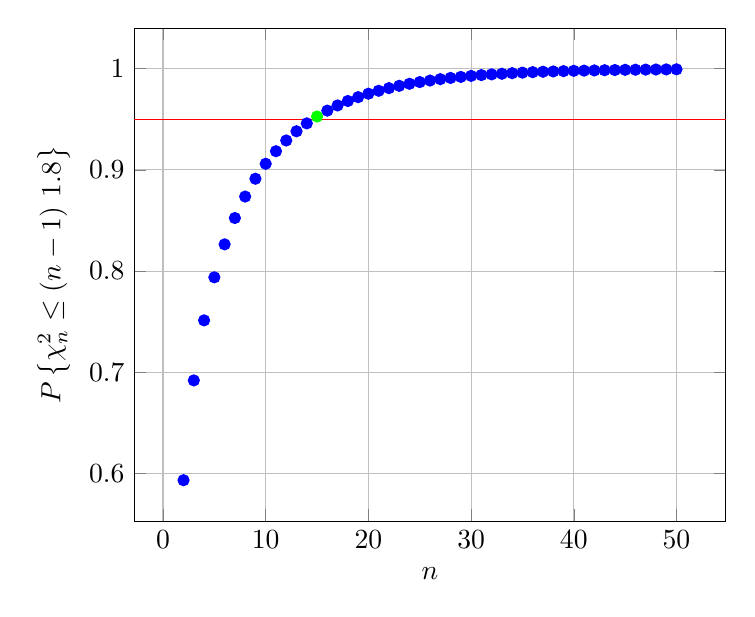
\begin{tikzpicture}
			\begin{axis}[width = 0.75\textwidth,xlabel=$n$, ylabel=$ P \left\{\chi_n^2 \leq (n-1)\ 1.8 \right\}  $, grid = both]
				
				\addplot[only marks, color = blue] plot coordinates{(2.0, 0.5934) (3.0, 0.692) (4.0, 0.7513) (5.0, 0.7938) (6.0, 0.8264) (7.0, 0.8524) (8.0, 0.8736) (9.0, 0.8912) (10.0, 0.906) (11.0, 0.9184) (12.0, 0.929) (13.0, 0.9381) (14.0, 0.9459) (16.0, 0.9585) (17.0, 0.9636) (18.0, 0.968) (19.0, 0.9718) (20.0, 0.9752) (21.0, 0.9781) (22.0, 0.9807) (23.0, 0.983) (24.0, 0.985) (25.0, 0.9867) (26.0, 0.9882) (27.0, 0.9896) (28.0, 0.9908) (29.0, 0.9918) (30.0, 0.9928) (31.0, 0.9936) (32.0, 0.9943) (33.0, 0.9949) (34.0, 0.9955) (35.0, 0.996) (36.0, 0.9965) (37.0, 0.9969) (38.0, 0.9972) (39.0, 0.9975) (40.0, 0.9978) (41.0, 0.998) (42.0, 0.9982) (43.0, 0.9984) (44.0, 0.9986) (45.0, 0.9988) (46.0, 0.9989) (47.0, 0.999) (48.0, 0.9991) (49.0, 0.9992) (50.0, 0.9993)};
				
				\addplot[only marks, color = green] plot coordinates{(15.0, 0.9527)};
			
				\draw [draw=red] (axis cs: -5,0.95) -- (axis cs: 60,0.95);
			\end{axis}
		\end{tikzpicture}
	\end{figure}

	\item Two samples with $ n_1 = 10, \sigma^2_1  = 4$ and $ n_2 = 5, \sigma^2_2  = 2$ \\
	
	\begin{subequations}
		\begin{align}
			\frac{S_1^2}{\sigma_1^2} &= \frac{\chi_9^2}{9} \qquad \frac{S_2^2}{\sigma_2^2} = \frac{\chi_4^2}{4} \nonumber \\
			%
			\frac{S_2^2}{S_1^2} &\geq 1 \qquad F_{4, 9} \geq 2 \nonumber \\
			%
			P  \left\{\frac{S_2^2}{S_1^2}  \geq 1\right\}  &= P \left\{F_{4, 9} \geq 2\right\}= 0.1782
 		\end{align}\\
	\end{subequations}
	
	\item $ n = 100, p  = 0.12$. Using the normal RV approximation with $ \mu = np = 12 $ and $ \sigma^2 = np(1-p)$ \\
	
	\begin{subequations}
		\begin{align}
			P \left\{9.5 \leq X \leq 14.5 \right\} &= P \left\{\frac{(9.5 - 12)}{\sqrt{12*0.88}} \leq Z \leq \frac{(14.5 - 12)}{\sqrt{12*0.88}} \right\} \nonumber \\
			%
			&= \Phi  \left(\frac{(14.5 - 12)}{\sqrt{12*0.88}}\right) - \Phi  \left(\frac{(9.5 - 12)}{\sqrt{12*0.88}}\right)  \nonumber \\
			%
			&= 0.5583
		\end{align}\\
	\end{subequations}

	\item Each human is a binomial RV with $ p = 0.52 $. Let $ n $ vary and check probability including continuity correction\\
	\begin{subequations}
		\begin{align}
			P \left\{ X \geq 0.5n \right\} &= P \left\{ Z \geq \frac{0.5n - 0.52n - 0.5}{\sqrt{np(1-p)}} \right\} \\
			%
			n = 10 &\to P = 0.6711 \nonumber \\
			%
			n = 100 &\to P = 0.6916 \nonumber \\
			%
			n = 1000 &\to P = 0.9028 \nonumber \\
			%
			n = 10000 &\to P = 0.99997 \nonumber 
		\end{align}\\
	\end{subequations}

	\item $ n = 300 $ men. $ c = 0.454, b = 0.284 $ \\
	\begin{subequations}
		\begin{enumerate}
			\item 			
			\begin{align}
				P \left\{X \geq 150 \right\} &= P \left\{Z \geq \frac{149.5 - 136.2}{\sqrt{300*0.454*0.546}} \right\} \nonumber \\
				%
				&= 0.0615
			\end{align} \\
			
			\item 
			\begin{align}
				P \left\{Y \leq 100 \right\} &= P \left\{Z \leq \frac{100.5 - 85.2}{\sqrt{300*0.284*0.716}} \right\} \nonumber \\
				%
				&= 0.9749
			\end{align} \\
			
		\end{enumerate}
	\end{subequations}

	\item $ n = 300 $ women. $ d = 0.256, a = 0.214 $ \\
	\begin{subequations}
		\begin{enumerate}
			\item 			
			\begin{align}
				P \left\{V \geq 60 \right\} &= P \left\{Z \geq \frac{59.5 - 76.8}{\sqrt{300*0.256*0.744}} \right\} \nonumber \\
				%
				&= 0.9889
			\end{align} \\
			
			\item 
			\begin{align}
				P \left\{U \leq 50 \right\} &= P \left\{Z \leq \frac{50.5 - 64.2}{\sqrt{300*0.214*0.786}} \right\} \nonumber \\
				%
				&= 0.0269
			\end{align} \\
			
		\end{enumerate}
	\end{subequations}

	\item More women than men rarely eat breakfast.\\
	 $ \mathbb{E}[X-Y] = -10.2 $, and $\mathrm{Var}(X-Y) = 147.4452$\\
	\begin{subequations}
		\begin{align}
			P \left\{X > Y \right\} &= P \left\{ X - Y > 0 \right\} \nonumber \\
			%
			&= P \left\{ Z > \frac{0 + 10.2}{\sqrt{147.4452}}  \right\} = 0.2005
		\end{align} \\
	\end{subequations}

	\item $ n = 1000 $ , $ p $ from the table as necessary. \\
	\begin{subequations}
		\begin{enumerate}
			\item 			
			\begin{align}
				P \left\{A \geq 500 \right\} &= P \left\{Z \geq \frac{500 - 542}{\sqrt{248.236}} \right\} \nonumber \\
				%
				&= 1 - \Phi \left( \frac{500 - 542}{\sqrt{248.236}} \right) = 0.9962
			\end{align} \\
			
			\item 
			\begin{align}
				P \left\{B > 500 \right\} &= P \left\{Z > \frac{500 - 704}{\sqrt{208.384}} \right\} \nonumber \\
				%
				&= 1 - \Phi \left( \frac{500 - 704}{\sqrt{208.384}} \right) \approx 1
			\end{align} \\
		
			\item 
			\begin{align}
				P \left\{C > 500 \right\} &= P \left\{Z > \frac{500 - 458}{\sqrt{248.236}} \right\} \nonumber \\
				%
				&= 1 - \Phi \left( \frac{500 - 458}{\sqrt{248.236}} \right) = 0.00384 \nonumber \\
				%
				P\left\{ \text{required} \right\} &= 0.00384 * 1 = 0.00384
			\end{align} \\
		
			\item 
			\begin{align}
				P \left\{D < 250 \right\} &= P \left\{Z < \frac{250 - 293}{\sqrt{207.151}} \right\} \nonumber \\
				%
				&= \Phi \left( \frac{250 - 293}{\sqrt{207.151}} \right) = 0.0014
			\end{align} \\
		
			\item 
			\begin{align}
				P \left\{E \geq 200 \right\} &= P \left\{Z \geq \frac{200 - 149}{\sqrt{126.799}} \right\} \nonumber \\
				%
				&= 1 - \Phi \left( \frac{200 - 149}{\sqrt{126.799}} \right) \approx 0
			\end{align} \\
		
			\item Let $ F = F_1 - F_2 $, with $ \mathbb{E}[F] = 31$, $ \mathrm{Var}[F] = 253.819$
			\begin{align}
				P \left\{F_1 - F_2 \geq 0 \right\} &= P \left\{Z \geq \frac{0 - 31}{\sqrt{253.819}} \right\} \nonumber \\
				%
				&= 1 - \Phi \left( \frac{0 - 31}{\sqrt{253.819}} \right) = 0.9742
			\end{align} \\
			
		\end{enumerate}
	\end{subequations}

	\item Each worker belongs to a union where $ p = 0.105 $ with $ n = 5 $. The older value of $ q = 0.201 $\\
	$ \mathbb{E}[X-Y] = -10.2 $, and $\mathrm{Var}(X-Y) = 147.4452$\\
	\begin{subequations}
		\begin{align}
			P \left\{X = 0 \right\} &= (1-p)^5 = 0.5743 \\
			%
			P \left\{Y = 0 \right\} &= (1-q)^5 = 0.3256
		\end{align} \\
	\end{subequations}

	\item $ n = 144 $ women. $ \mu = 517, \sigma = 120 $ \\
	\begin{subequations}
		\begin{enumerate}
			\item 			
			\begin{align}
				P \left\{\overline{X} > 507 \right\} &= P \left\{Z > \frac{507 - 517}{120/12} \right\} \nonumber \\
				%
				&= 1 - \Phi (-10/10) = 0.8413
			\end{align} \\
			
			\item 			
			\begin{align}
				P \left\{\overline{X} > 517 \right\} &= P \left\{Z > \frac{517 - 517}{120/12} \right\} \nonumber \\
				%
				&= 1 - \Phi (0/10) = 0.5
			\end{align} \\
		
		
			\item 			
			\begin{align}
				P \left\{\overline{X} > 537 \right\} &= P \left\{Z > \frac{537 - 517}{120/12} \right\} \nonumber \\
				%
				&= 1 - \Phi (20/10) = 0.0227
			\end{align} \\
		
			\item 			
			\begin{align}
				P \left\{\overline{X} > 550 \right\} &= P \left\{Z > \frac{550 - 517}{120/12} \right\} \nonumber \\
				%
				&= 1 - \Phi (33/10) = 0.00048
			\end{align} \\
			
		\end{enumerate}
	\end{subequations}
	
	\item $ n = 12 $ women. $ \mu = 53600, \sigma = 3200 $ \\

	\begin{subequations}
		\begin{align}
			P \left\{\overline{X} > 55000 \right\} &= P \left\{Z > \frac{55000 - 53600}{3200/\sqrt{12}} \right\} \nonumber \\
			%
			&= 0.0648
		\end{align} \\
	\end{subequations}

	\item $ n = $ is to be found. $ \mu = 100, \sigma = 30 $. Let $ Y = \sum X_i $ \\
	
	\begin{subequations}
		\begin{align}
			P \left\{Y > 2000 \right\} &= P \left\{Z > \frac{2000 - 100\ n}{30\ \sqrt{n}} \right\} \geq 0.95 \nonumber \\
			%
			\Phi \left( \frac{2000 - 100\ n}{30\ \sqrt{n}} \right) &\leq 0.05 \nonumber \\
			%
			2000 - 100\ n &\leq -1.6448 \times 30\sqrt{n} \nonumber \\
			%
			n &\geq 23
		\end{align} \\
	
	\begin{figure}[H]
		\centering
		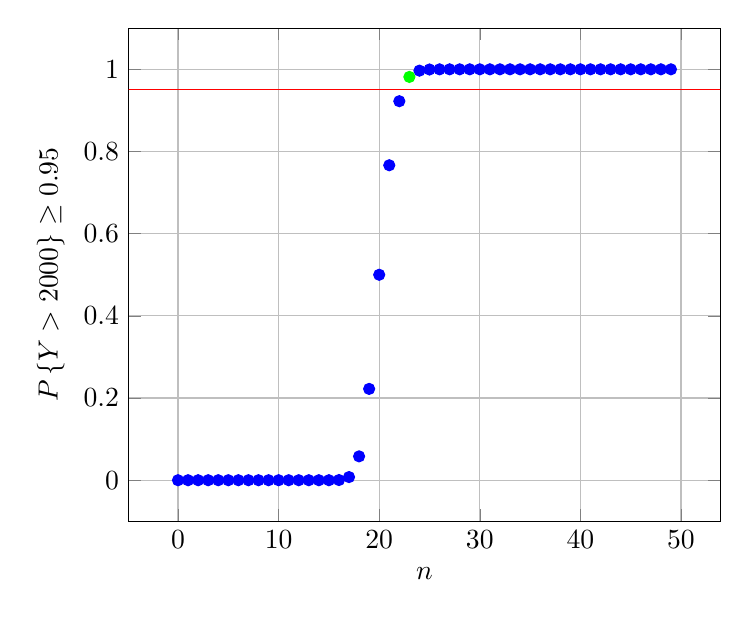
\begin{tikzpicture}
			\begin{axis}[width = 0.75\textwidth,xlabel=$n$, ylabel=$ P \left\{ Y > 2000 \right\} \geq 0.95  $, grid = both]
				
				\addplot[only marks, color = blue] plot coordinates{(0.0, 0.0) (1.0, 0.0) (2.0, 0.0) (3.0, 0.0) (4.0, 0.0) (5.0, 0.0) (6.0, 0.0) (7.0, 0.0) (8.0, 0.0) (9.0, 0.0) (10.0, 0.0) (11.0, 0.0) (12.0, 6.8833827526759706e-15) (13.0, 4.851663515381688e-11) (14.0, 4.5152443450824364e-08) (15.0, 8.413074170987578e-06) (16.0, 0.0004290603331967846) (17.0, 0.007646685515099505) (18.0, 0.058050871990274366) (19.0, 0.2222194112520176) (20.0, 0.5) (21.0, 0.7665073693266079) (22.0, 0.922390755157658) (24.0, 0.9967522068714105) (25.0, 0.9995709396668032) (26.0, 0.999956150288122) (27.0, 0.9999964472261701) (28.0, 0.9999997666572595) (29.0, 0.9999999873257626) (30.0, 0.9999999994204671) (31.0, 0.9999999999773364) (32.0, 0.9999999999992313) (33.0, 0.9999999999999771) (34.0, 0.9999999999999994) (35.0, 1.0) (36.0, 1.0) (37.0, 1.0) (38.0, 1.0) (39.0, 1.0) (40.0, 1.0) (41.0, 1.0) (42.0, 1.0) (43.0, 1.0) (44.0, 1.0) (45.0, 1.0) (46.0, 1.0) (47.0, 1.0) (48.0, 1.0) (49.0, 1.0)
				};
				
				\addplot[only marks, color = green] plot coordinates{(23.0, 0.9814718907179405)};
				
				\draw [draw=red] (axis cs: -5,0.95) -- (axis cs: 60,0.95);
			\end{axis}
		\end{tikzpicture}
	\end{figure}
	\end{subequations}
\end{enumerate}